% This template was initially provided by Dulip Withanage.
% Modifications for the database systems research group
% were made by Conny Junghans,  Jannik Strötgen and Michael Gertz

\documentclass[
     12pt,         % font size
     a4paper,      % paper format
     BCOR10mm,     % binding correction
     DIV14,        % stripe size for margin calculation
     ]{article}

%%%%%%%%%%%%%%%%%%%%%%%%%%%%%%%%%%%%%%%%%%%%%%%%%%%%%%%%%%%%

% PACKAGES:

% Use German
\usepackage[english]{babel}
% Input and font encoding
\usepackage[latin1]{inputenc}
\usepackage[T1]{fontenc}
% Index-generation
\usepackage{makeidx}
% Embedding of URLs
\usepackage{url}
% Special \LaTex symbols (e.g. \BibTeX)
%\usepackage{doc}
% Include Graphic-files
\usepackage{graphicx}
% Include doc++ generated tex-files
%\usepackage{docxx}
% Fuer anderthalbzeiligen Textsatz
\usepackage{setspace}
\usepackage[table,xcdraw]{xcolor}
\usepackage{hhline}
\usepackage{highlight}

\usepackage{subcaption}

\usepackage{biblatex}
\bibliography{references.bib}

% hyperrefs in the documents
\PassOptionsToPackage{hyphens}{url}\usepackage[bookmarks=true,colorlinks,pdfpagelabels,pdfstartview = FitH,bookmarksopen = true,bookmarksnumbered = true,linkcolor = black,plainpages = false,hypertexnames = false,citecolor = black,urlcolor=black]{hyperref}
%\usepackage{hyperref}


% CUSTOM:

% For quotes:
\usepackage{csquotes}

% For Definitions:                   						
\usepackage{amsthm}
\usepackage[framemethod=tikz]{mdframed}

\newtheoremstyle{defi}
{\topsep}         % Abstand oben
{\topsep}         % Abstand unten
{\normalfont}     % Schrift des Bodys
{0pt}             % Einschub der ersten Zeile
{\bfseries}       % Darstellung von der Schrift in der �berschrift
{:}               % Trennzeichen zwischen �berschrift und Body
{.5em}            % Abstand nach dem Trennzeichen zum Body Text
{\thmname{#3}}    % Name in eckigen Klammern
\theoremstyle{defi}

\newmdtheoremenv[
hidealllines = true,       % Rahmen komplett ausblenden
leftline = true,           % Linie links einschalten
innertopmargin = 0pt,      % Abstand oben
innerbottommargin = 4pt,   % Abstand unten
innerrightmargin = 0pt,    % Abstand rechts
linewidth = 3pt,           % Linienbreite
linecolor = gray!40,       % Linienfarbe
]{defStrich}{Definition}     % Name der des formats "defStrich"



%%%%%%%%%%%%%%%%%%%%%%%%%%%%%%%%%%%%%%%%%%%%%%%%%%%%%%%%%%%%

% OTHER SETTINGS:

% Choose language
\newcommand{\setlang}[1]{\selectlanguage{#1}\nonfrenchspacing}


\begin{document}

% TITLE:
\pagenumbering{roman} 
\begin{titlepage}

\vspace*{1cm}
\begin{center}
\textbf{ 
\Large Heidelberg University\\
\smallskip
\Large Institute of Computer Science\\
\smallskip
\Large Database Systems Research Group\\
\smallskip
}

\vspace{3cm}

\textbf{\large Report for the lecture Text Analytics}

\vspace{0.5\baselineskip}
{\huge
\textbf{Hate Speech Detection}
}
\vspace{0.5cm}

\url{https://github.com/fidsusj/HateSpeechDetection}

\vspace{1cm}
Mentor: John Ziegler
\end{center}

\vfill 

{\large
\begin{tabular}[l]{ll}
Team Member: & Christopher Klammt, 3588474,\\
  & Applied Computer Science\\
  & iv249@stud.uni-heidelberg.de\\
  & \\
Team Member: & Felix Hausberger, 3661293,\\
  & Applied Computer Science\\
  & eb260@stud.uni-heidelberg.de\\
  & \\
Team Member: & Nils Krehl, 3664130,\\
  & Applied Computer Science\\
  & pu268@stud.uni-heidelberg.de\\
  
\end{tabular}
}

\end{titlepage}

\pagenumbering{arabic}

\section*{Abstract}

\section*{Plagiarism statement}

We certify that this report is our own work, based on our personal study and/or research and that we have acknowledged all material and sources used in its preparation, whether they be books, articles, reports, lecture notes, and any other kind of document, electronic or personal communication.
We also certify that this report has not previously been submitted for assessment in any other unit, except where specific permission has been granted from all unit coordinators involved, or at any other time in this unit, and that we have not copied in part or whole or otherwise plagiarized the work of other students and/or persons.


\newpage
\tableofcontents
\newpage

\section{Introduction}

One current research area in the field of text analytics is hate speech detection. Many approaches from the recent past take use of neural network architectures to deal with such classification problems. One of the most common approaches is to use uni- and bidirectional long short-term memory (LSTM) networks, a recurrent neural network architecture that can process input of arbitrary length and remembers context information \cite{Dorris2020, Syam2019, Saksesi2018}. The paper \cite{Founta2019} states, that even a simple gated recurrent unit (GRU) architecture can perform as good as more complex units. \cite{Saleh2020} repurposes the famous bidirectional encoder representations from transformers (BERT) language model to perform classification tasks for hate speech detection. Besides that, other approaches use convolutional neural networks (CNNs) to extract typical hate speech patterns \cite{Badjatiya2017, Roy2020, Kapil2020} or even deep belief network algorithms \cite{Muhammad2020}. Using neural network approaches means to automatically learn representative features for the classification task. On the other hand, the papers introduced in \autoref{related_work} use a different approach by solving the classification task with manually extracted features. Nevertheless, none of the papers combines the different achievements of such recent research and compares it to a baseline neural network architecture, which is what this work is dedicated to.

After a definition of the term \enquote{hate speech} in \autoref{approach} different classifiers will be trained on a holistic, hand-crafted feature set based on recent publications in the field of hate speech detection. The task includes building and preprocessing a training corpus as well as introducing and explaining the different kinds of features. How well the different classifiers perform compared to a neural network approach as a baseline and several statictical insights into typical hate speech artifacts will be presented in \autoref{results}. The results of this work in \autoref{analysis} should show which features work best for which classifier and which problems can be addressed with conventional machine learning methods and which not as opposed to neural network approaches. A summary over the achievements earned will be drawn in \autoref{conclusion}.
\newpage
\section{Related Work} \label{related_work}

As the goal of this work is to solve a hate speech classification problem with manually extracted features, recent work was evaluated proposing different feature sets for this task. 

\cite{Watanabe2018} categorizes features into four different groups. Sentiment-based fea\-tures give information about the polarity of a document, which is important as many hate speech documents stand out by being mostly negativ. Sentiment features count the occurences of punctuations, capitalized words, interjections, etc. A dictionary of typical hate speech words can be obtained by extracting most common unigrams from a given corpus building the unigram features. Pattern features represent the last feature group containing common syntactic patterns based on PoS tags. The approach presented in this paper achieved an accuracy of 87.4\% using combined features from these four groups. The classifiers used were SVM, Random Forest and J48graft.

\cite{Oriola2020} concludes character n-grams, word n-grams, negative sentiment-based scores and syntactic-based features as a decent feature set to train classifiers on. Looking at the results, an optimized support vector machine with character n-grams performed best with 0.894 TPR, while optimized gradient boosting performed best with word n-grams, giving a 0.867 TPR. 

\cite{Fortuna2018} divides features into generic text mining features and specific hate speech detection features. Typical generic text mining features are dictionaries of insults typical for heate speech, swear words, profane words, verbal abuse etc., n-grams, lexical syntactic based template features, that capture gram\-mat\-i\-cal dependencies within a sentence, topic classifications with latent dirich\-let allocation, or sentiment polarity scores. On the other hand specific hate speech detection features do not rely on common abstract concepts known in the field of text analytics, but come with purpose built frameworks to detect these featues. Using the Stanford lexical parser along with a context-free lexical parsing model one can identify language which is used a lot in hate speech. Other examples of specific hate speech features are the objectivity-subjectivity relations of the language as hate speech is more related to subjective communication, focus on particular stereotypes, in\-ter\-sec\-tion\-ism of oppression or declarations of superiority of the ingroup. 

Other related work like \cite{Gaydhani2018}, \cite{Malmasi2017} and \cite{ThomasDavidson2020} once more stress the importance of word and character n-grams for hate speech detection tasks. \cite{ThomasDavidson2020} even uses count indicators for hashtags, mentions, retweets and URLs and is especially important as a part of the dataset used in this work originated from the project behind this paper. The best performing model achieved 91\% overall precision, 90\% recall and a 90\% F1-score, but the model is biased towards classifying tweets as less hateful or offensive than the human supervisors. 

\section{Approach} 
\label{approach}

The epistemic research interest in this work is to clarify the question, whether conventional machine learning methods combined with suitable features can outperform neural network based approaches.

\begin{figure}[ht]
	\centering
	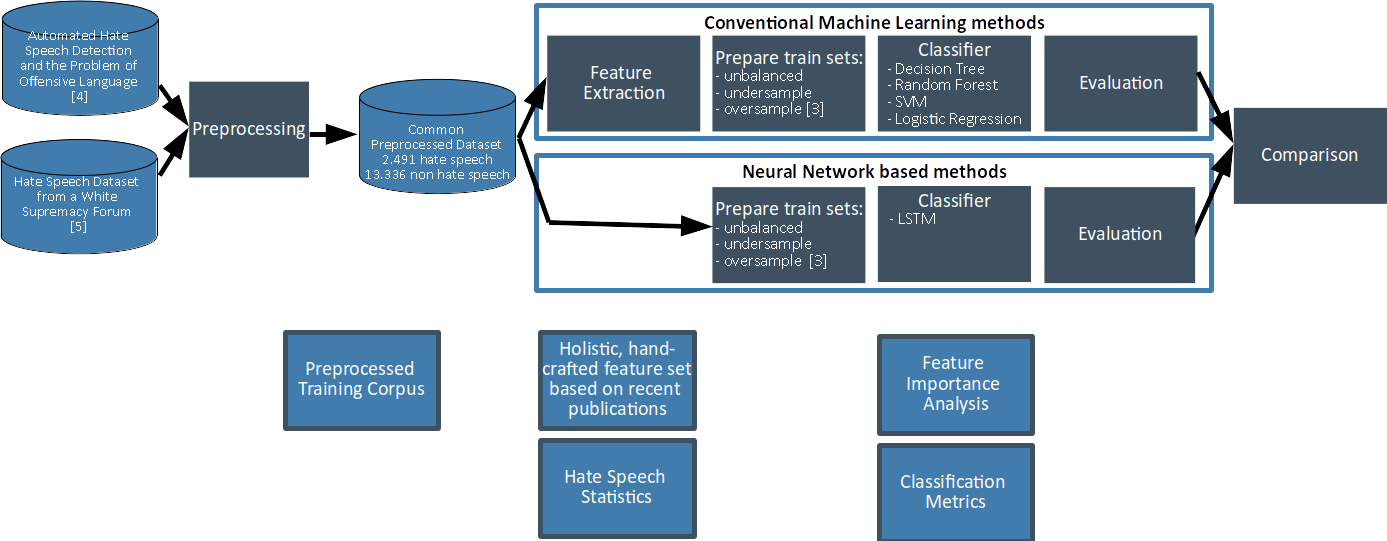
\includegraphics[width=1.0\linewidth]{figures/pipeline.png}
	\caption{Approach}
	\label{fig:overall_pipeline}
\end{figure}

Figure \ref{fig:overall_pipeline} visualizes our approach (on the top) and the resulting novelties achieved through this work (at the bottom). The following chapters describe the different steps in detail. First the data is merged and preprocessed resulting in a preprocessed training corpus. The next step differs between conventional machine learning methods and neural network based approaches. For conventional machine learning methods an explicit feature extraction is necessary. Therefore achievements of recent publications were combined to build a holistic, hand-crafted feature set. Based on these features, hate speech statistics could be further analyzed. Due to the fact that the common preprocessed corpus is unbalanced, an unbalanced, oversampled and undersampled dataset was created for further investigation. Finally the classifiers are trained, evaluated and the results are compared. Now not only the question whether conventional machine learning methods can outperform neural network based approaches could be answered, but as well which feature were most important for which classifier.

\subsection{Definition of Hate Speech} 
\label{ch:approachA}

Various definitions exist to define hate speech. This work complies with the definitions provided by the two datasets used to label the documents. 

\begin{defStrich}[Ona De Gibert et al.]
	Hate speech is commonly defined as any communication that disparages a target group of people based on some characteristic such as race, color, ethnicity, gender, sexual orientation, nationality, religion, or other characteristic \cite{DeGibert2020}.
\end{defStrich}

\begin{defStrich}[Thomas Davidson et al.]
	A language that is used to expresses hatred towards a targeted group or is intended to be derogatory, to humiliate, or to insult the members of the group \cite{ThomasDavidson2020}.
\end{defStrich}

One can conclude that hate speech is always targeted towards a specific group with the intention to infringe others dignity, often based on group characteristics like race, color or gender. 

\subsection{Data}
\label{ch:approachB}

There are two data sets used for the project. The first one uses data from the \textit{Twitter API} \cite{ThomasDavidson2020}\footnote{https://github.com/t-davidson/hate-speech-and-offensive-language}. It consists of a sample of around 25k tweets that were identified as hate speech based on a previously composed hate speech lexicon without regarding context information. Subsequently, each document in the corpus got labeled with one of the three categories \textit{hate speech}, \textit{offensive language} or \textit{neutral}. The workers were instructed to follow predefined definitions of each category and to take context information into consideration. Each tweet was assessed and labeled by three or more workers. The majority of tweets were classified as offensive language (76\% at 2/3, 53\% at 3/3), only 5\% were coded as hate speech. In the end 1.430 hate speech documents, 4.175 neutral documents and 19.196 offensive language documents make up the entire dataset. The data is provided offline as a CSV or pickle file. 

The second data set uses data from \textit{Stormfront}, a white supremacy forum \cite{DeGibert2020}\footnote{https://github.com/Vicomtech/hate-speech-dataset}. One document represents a sentence that is either labeled as hate or not hate. In total, 1.196 sentences containing hate and 9.507 sentences being non-hate are provided. Once again the documents were labeled manually by human actors following previously specified guidelines, on request additional context information was provided. The documents are given offline as normal text files with annotations stored in a separate CSV file. 

\subsection{Features}
\label{ch:approachC}

The choice of features to use can be divided into five groups inspired by \cite{Watanabe2018}. 

One group of features is the unigrams features group inspired by \cite{ThomasDavidson2020, Oriola2020, Fortuna2018, Gaydhani2018, Malmasi2017}. During the training phase we extract the top 100 words for hate speech and neutral speech based on the TFIDF scores. These words are given as dictionaries during the feature extraction phase. We therefore count the occurences of typical hate speech and neutral speech words in each document as a feature. A similar approach extracts typical hate speech n-grams based on word stems using with NLTK during the training phase and builds n-gram dictionaries. In case n-grams surpass a certain threshold they are added to the dictionary. This threshold is 10 for unigrams, 8 for bigrams and 2 for trigrams. The number of typical hate speech unigrams, bigrams and trigrams detected is added as a feature. 

Another feature group are the semantic features taken from \cite{ThomasDavidson2020, Watanabe2018}. They comprise the number of exclamation marks, question marks, full stop marks, interjections\footnote{recognized by NLTKs PoS tags}, all capital words, quotation marks as an approximation for the number of quotes, laughing expressions\footnote{based on the regular expression \textit{r"(a*ha+h[ha]*|o?l+o+l+[ol]*)|(lmao)"}} and the number of words in general. 

To expand the set of features to cover syntactical characteristics of hate speech documents, PoS tag patterns were extracted belonging to the group of pattern features \cite{Oriola2020, Fortuna2018}. A sliding window approach with a custom definable window size range is used to extract PoS tag patterns for each document during the training phase. In case a hate speech pattern occurs more than 500 times in the training set it is added to a hate speech pattern dictionary. The number of hate speech patterns detected in each document in taken as a feature.

Sentiment-based features inspired by \cite{Oriola2020, Fortuna2018} were implemented by extracting the polarity scores for each document using NLTKs SentimentIntensityAnalyzer from VADER (Valence Aware Dictionary and sEntiment Reasoner). VADER is a lexicon and rule-based sentiment analysis tool specifically developed for social media sentiment analysis. 

The last feature added to the holistic, hand-crafted feature set is the topic detected from gensims latent dirichlet allocation algorithm \cite{Fortuna2018}. For each document a numerical topic of either zero or one is added to the set of features based on which topic received the highest probability score. 

The feature extraction of the previously mentioned features is done within a reusable pipeline, which makes it easy to add new features. Each feature is implemented as a class following a predefined interface. By adding the feature class to a list in the \textit{Feature\-Extractor} the feature is automatically extracted as part of the pipeline. The pipelines input are raw text documents, stemmed documents, lemmatized documents and PoS tags each in its own dataframe column and the output is a dataframe containing all extracted features as numerical values.

\subsection{Classifiers}
\label{ch:approachD}

In this work five classifiers are compared on the different datasets (unbalanced, undersampled, oversampled). Four of them are conventional machine learning methods (Decision Tree, Random Forest, SVM, Logistic Regression) and one neural network based approach (LSTM).

Each classifier is trained on the training set and evaluated on the test set. So the same steps are necessary for each classifier. That is why a reusable pipeline is developed. The pipeline is developed with the open-closed principle in mind. It is open for extensions and closed for changes. So when adding a new classifier only a few lines of code need to be adapted and steps such as finding the optimal model through hyperparameter tuning and the evaluation are done automatically as part of the pipeline.

As the methods need it, there are slight differences between the training of the conventional machine learning methods and the neural network based approaches. Figure \ref{fig:classifier_pipeline} illustrates this.

\begin{figure}[ht]
	\centering
	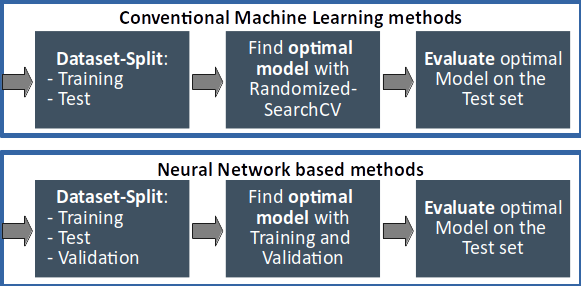
\includegraphics[width=0.7\linewidth]{figures/classifier_pipeline.png}
	\caption{Classifier pipeline}
	\label{fig:classifier_pipeline}
\end{figure}

For the conventional machine learning methods the dataset is split into training (0.8) and test set (0.2). In order to find the optimal model \textit{Randomized\-SearchCV} is executed on the defined hyperparameter search space. The hyperparameter search space was chosen based on the classifiers doc\-u\-men\-ta\-tion, papers and by an empirical examination. For the decision tree \cite{mantovani2019empirical} and for the random forest \cite{probstHyperparametersTuningStrategies2019} were observed. For SVM we used the sklearn C-Support Vector Classification implementation and concentrated the grid search on the kernel (linear, poly, rbf or sigmoid) as this has the biggest impact on performance. Tuning the kernel already used up quite some computational time, so we did not look into further parameters. In future work one could have a closer look at parameters such as the regularization parameter C or some kernel specific coefficients. To train the logistic regression model, hyperparameters were set according to the recommendations from sklearns documentation page. To try out different solver algorithms, the L2-norm penality for regularization was chosen. As the number of samples surpass the number of features the normal primal formulation of the regression problem was used. The search space for solver algorithms was restricted to \textit{lbfgs}, \textit{sag} and \textit{saga} as others did not make sense in the training circumstances. Also different regularization strength were tested with parameter C between 0.8 and 1.2 with step width 0.1. Finally the model is evaluated on the test set.

For neural network based approaches the dataset is again split into training (0.8) and test set (0.2). Then the training set is further split up into training (0.8) and validation (0.2). In the next step the optimal model is found by using the training and the validation set. The final step is equal to the final step in conventional machine learning, were the model is evaluated.

To enable a performant execution Pythons multiprocessing library is used to parallelize the execution.

\subsection{Evaluation}
\label{ch:approachE}

For evaluating the classifiers standard metrics such as accuracy, precision, recall and F1 score are used.

The accuracy specifies how many data instances are correctly classified. Only looking at the accuracy, is not that informative, because generally a lot of instances are correctly classified as non hate speech, which leads to a high accuracy. That is why also precision and recall are observed. Precision specifies how many of the predicted hate speech instances are really hate speech. A low precision means that many instances are classified as hate speech, although they are not. So looking at the precision enables us to detect if the trained model could be used as a censoring system and undermine the freedom of speech. The recall specifies how many hate speech instances are correctly classified by the model. A low recall means that there are many false negatives (a lot of hate speech instances are not detected). For taking into account precision and recall one can look at the F1 score.


\section{Experimental setup and results}

\section{Analysis} \label{analysis}

For answering our research question, whether classical Machine Learning methods combined with suitable features can outperform neural network based approaches, the following results were achieved:
\begin{itemize}
	\item Investigation of feature importances (chapter \ref{ch:experimentDa})
	\item Hate speech statistics (chapter \ref{ch:experimentDb})
	\item Comparison of the classifier results (classical Machine Learning methods vs neural network based approaches) (chapter \ref{ch:experimentDc})
	\item Oversampled and undersampled datasets (chapter \ref{ch:experimentDd})
\end{itemize}

\subsection{Feature importances}
\label{ch:experimentDa}


\subsection{Hate speech statistics}
\label{ch:experimentDb}

After extracting all the features, we had a closer look at them to identify which features are characteristic for hate speech.
Firstly, the semantic features in general do not signify whether a post is hate speech or not. Neither the number of exclamation marks, question marks, full stop marks, interjections or all caps words show any sign of signifying hate speech. These features are evenly distributed regarding hate speech versus non-hate speech.
The only semantic features which indicate hate speech are the number of words and - to a very small degree - the number of laughing expressions.
As already mentioned in \autoref{sec:data_analysis} the more words a post consists of, the likelier it is to be classified as hate speech (illustrated in \autoref{fig:wordclouds}).
Although, there are only very few laughing expressions identified per post (most do not contain any), there is a tendency for hate speech posts to contain more laughing expressions, such as \enquote{haha}, \enquote{lol} or similar.

Slightly more telling is the topic feature we trained using LDA with only 2 topics. It seems to have somewhat trained to classify into hate and non-hate - as we hoped. The hate speech posts are more likely to be classified as topic 0 than non-hate speech posts. But this difference is not really significant.

A more interesting and characteristic feature seems to be sentiment-based. As described, we extracted a sentiment-score (polarity) for each post using vader and this clearly differentiates between hate speech and non-hate speech, as shown in \autoref{fig:statistics_sentiment}.
This shows, that a negative sentiment-score indicates a post being rather likely to contain hate speech. The more positive the sentiment-score is, the less probable it is classified as hate speech.

\begin{figure}[ht]
	\centering
	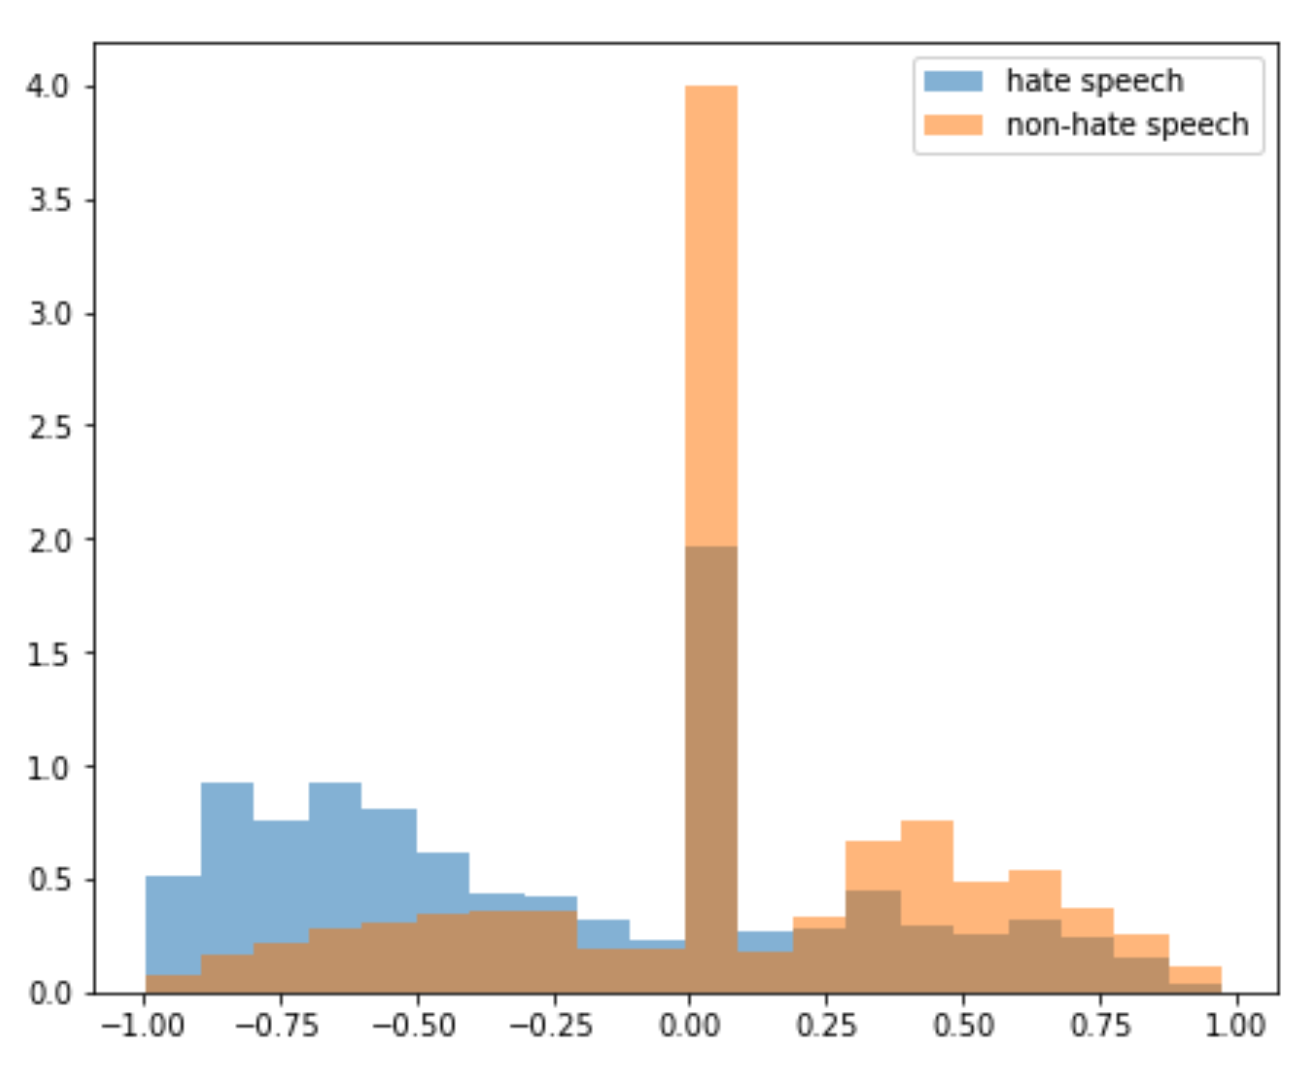
\includegraphics[width=0.7\linewidth]{figures/statistics_sentiment.png}
	\caption{Normalized distribution of sentiment score for hate speech vs. non-hate speech}
	\label{fig:statistics_sentiment}
\end{figure}

Further meaningful features were found using a dictionary approach by using the training data to generate a dictionary for hate speech and neutral words. The number of hateful words is distributed such that hate speech posts contain significantly more, whereas the number of neutral words does not differ much.
Examples for the most common hateful words found in hate speech posts are \enquote{fag}, \enquote{bitch}, \enquote{ass} or \enquote{nigga}. These words basically did not occur in non-hate speech posts. The most common neutral words are less informative, as the suffixes \enquote{ll} and \enquote{ve} are the most common ones for hate speech and non-hate speech posts.

Furthermore, we had an extensive look at unigrams, bigrams and trigrams for hate speech and these are significantly overrepresented in hate speech posts compared to non-hate speech posts. This especially holds true for the unigrams such as \enquote{white} which appears in 15\% of hate speech posts or \enquote{not} appearing in 9\% of hate speech posts. Both of these appear only half as often in non-hate speech posts.
The identified bigrams only show up in a very small percentage of posts, but significantly less in non-hate speech posts. Most common bigrams for hate speech are \enquote{white trash}, \enquote{look like} and \enquote{ass nigga}.

Lastly, the feature pattern-count can somewhat indicate hate speech, as the mean amount is higher for hate speech compared to non-hate speech. As one can see in \autoref{fig:statistics_pattern_count} hate speech tends to contain more patterns (which of course were trained by using the hate speech data).

\begin{figure}[ht]
	\centering
	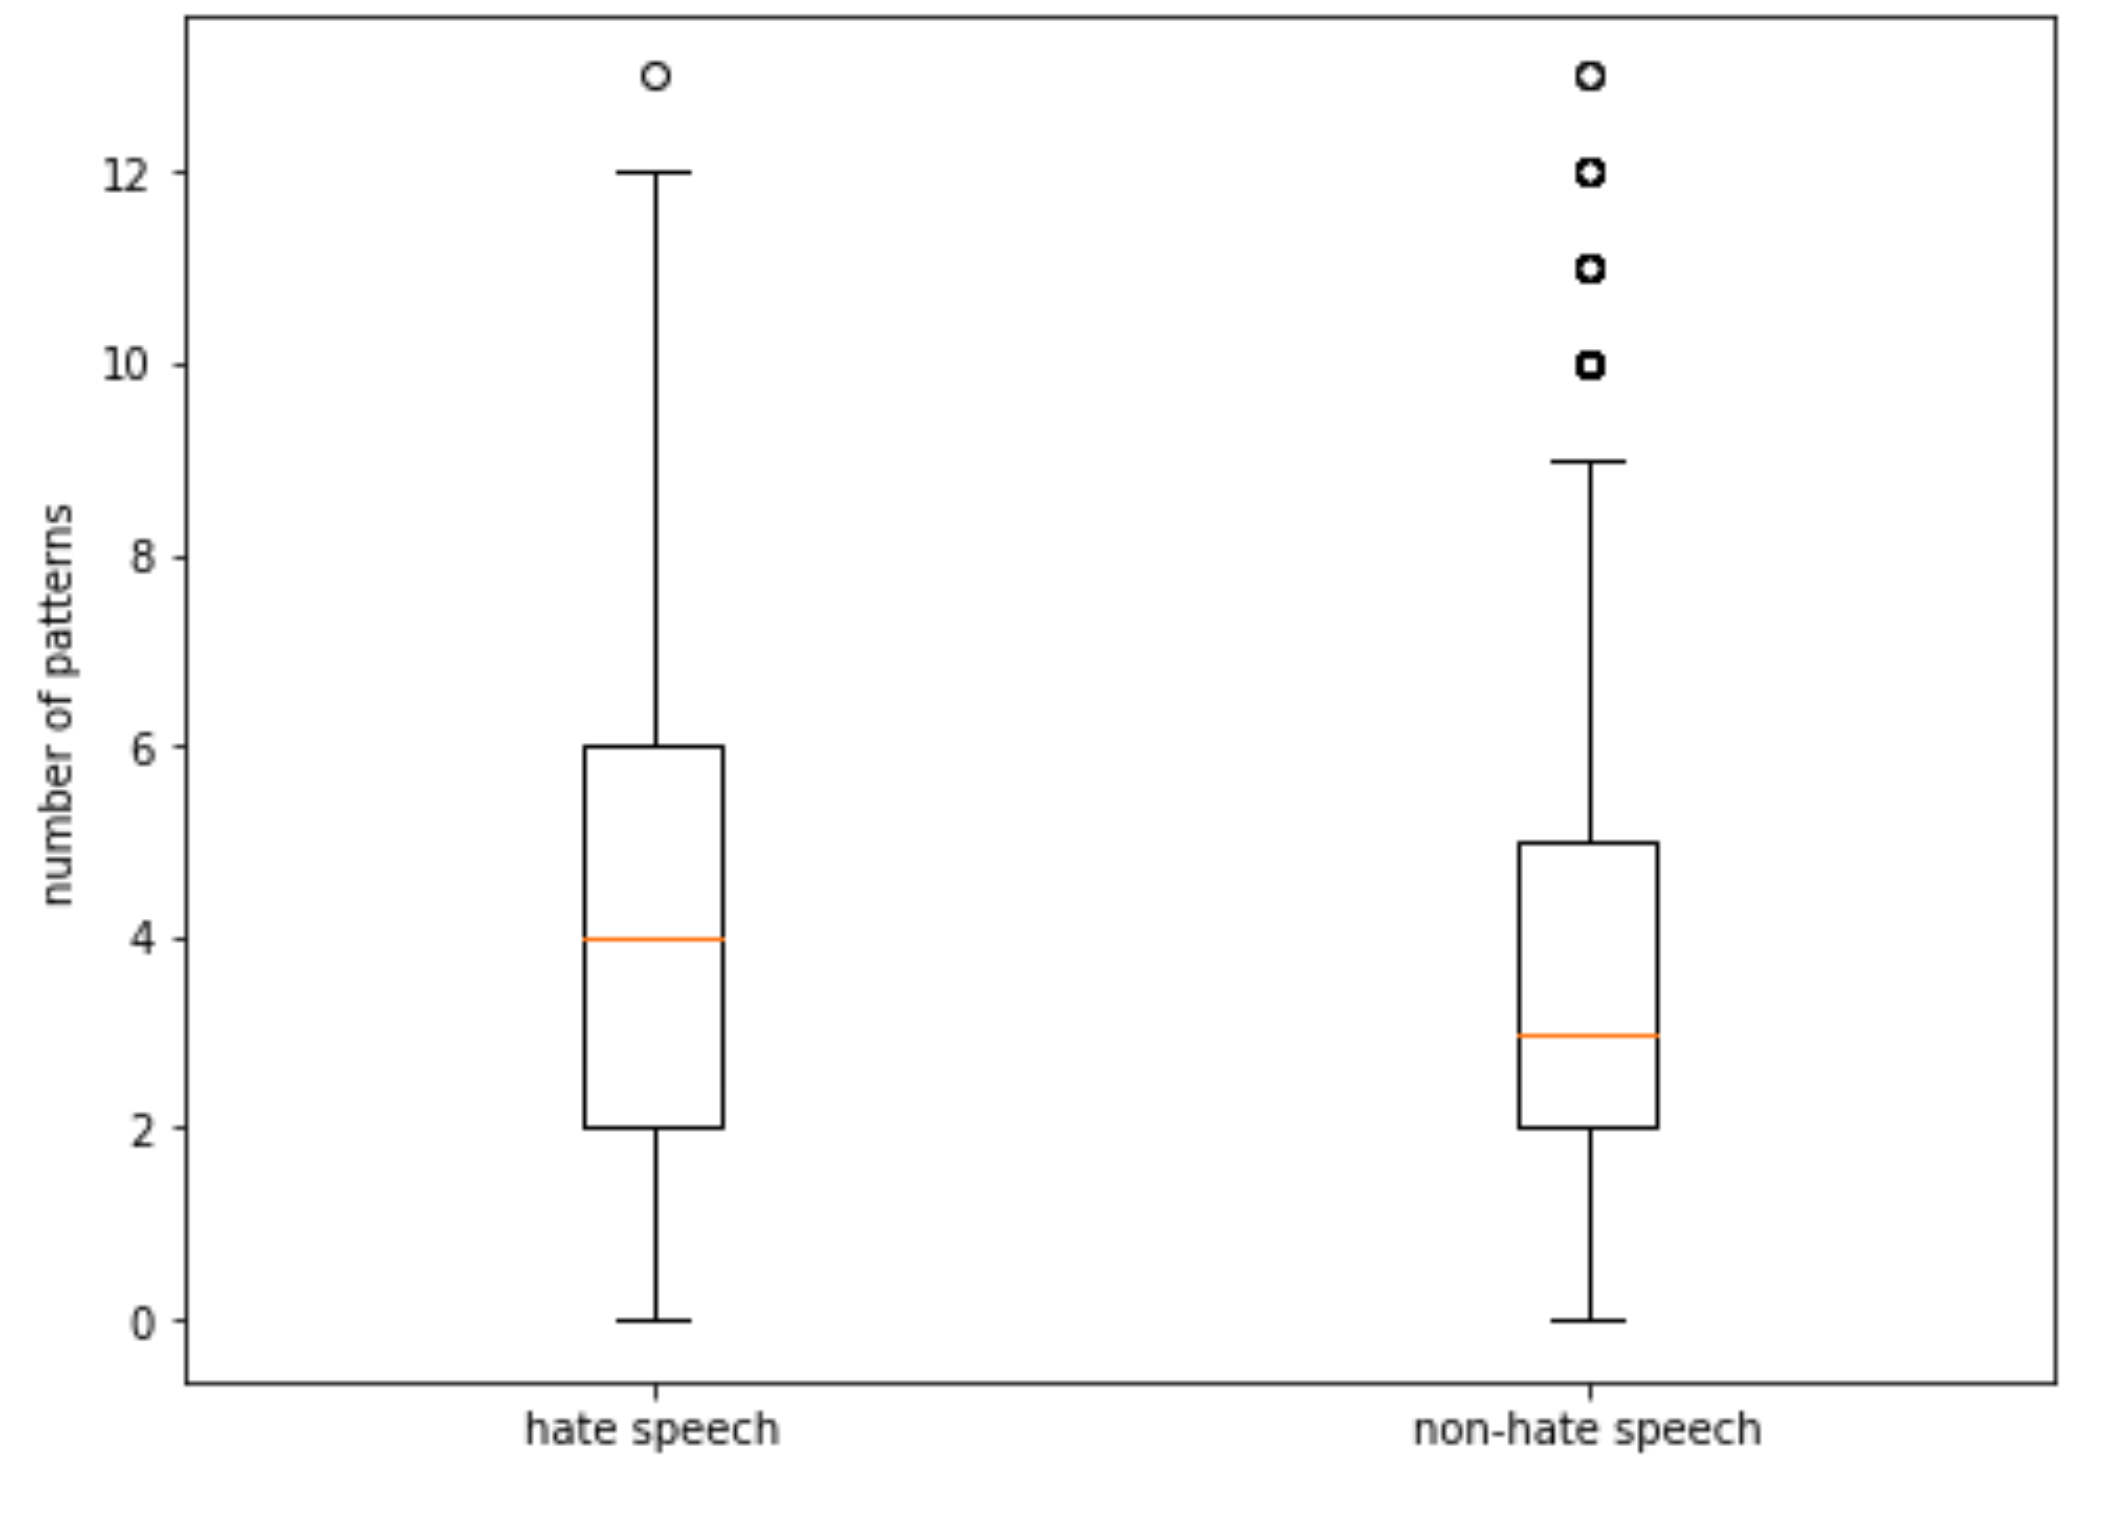
\includegraphics[width=0.7\linewidth]{figures/statistics_pattern_count.png}
	\caption{Boxplots comparing the number of patterns occurring in hate speech vs. non-hate speech}
	\label{fig:statistics_pattern_count}
\end{figure}

But maybe it would be worthwhile to have a closer look at the patterns and adjust them for some future work. Because when we look at single patterns, some occur more often in hate speech and some more often in non-hate speech (in our dataset). For example the pattern \enquote{adjective, noun (JJ, NN)} occurs in 56\% of hate speech and in 48\% of non-hate speech, whereas the pattern \enquote{determiner, noun} occurs in 5\% less hate speech posts than non-hate speech posts. So a more thorough analysis of these patterns could benefit this feature a lot, maybe by using individual features for each pattern. For example the biggest difference in occurrences is achieved by the pattern \enquote{personal pronoun, non-3rd person singular present verb (PRP, VBP)} with a 10\% difference.

\subsection{Comparison of the classifier results}
\label{ch:experimentDc}

All classifiers perform about equally well. And the achieved results are good with about 93\% for the F1-score. In the unbalanced case the conventional Machine Learning methods can definitely keep up with the neural network baseline. 

\subsection{Oversampled and undersampled datasets}
\label{ch:experimentDd}

In the undersampled case all conventional Machine Learning methods perform about equally well. Compared to the results from unbalanced dataset the conventional classifiers perform worse. In contrast the neural network baseline can keep up with the results from the unbalanced case. So in this undersampled case the conventional Machine Learning methods cannot keep up with the neural network baseline.

In the oversampled case the results are located between the undersampled and the unbalanced case. An outstanding result is the Random Forest, which performs better then the other conventional Machine Learning methods. As already mentioned SMOTE is not able to generate new textual features for generating an oversampled dataset for the neural network baseline. That is why these results could not be measured.

\section{Conclusion} \label{conclusion}

Coming to a conclusion, our main research question was whether conventional machine learning approaches combined with suitable features can outperform neural network based approaches. The short answer to this is, that the classical machine learning methods based on our hand-crafted feature set are definitely able to compete with our neural network baseline. For the unbalanced dataset the LSTM baseline only slightly - and rather insignificantly - outperforms the different classical methods, which all perform quite similarly. They also perform quite well with an F1-score around 93\%. But it is important to note, that we used randomized search to optimize these methods by tuning the hyperparameters, so there is not much room for improvement. For our neural network approach this does not hold true, as we only used a basic implementation without much fine-tuning or testing different network architectures.

Furthermore, while answering this research question we also created a common hate speech dataset from \cite{ThomasDavidson2020} and \cite{DeGibert2020} and a solid hand-crafted feature set based on recent publications upon it. We also developed an easily extendible pipeline incorporating the preprocessing of the underlying data as well as making it easy to add more features and classifiers.

Another finding of our work is the insights into the hate speech statistics and feature importance which lets us have a look at what hate speech is "made" of and indicators for it. The most important features are sentiment and unigram features, with a few words that clearly indicate hate.

\vspace{0.5cm}

As an outlook, there are some improvements and further investigations we would like to evaluate in future work. For one it should be very interesting to expand the currently binary classification into hate speech and non-hate speech to a ternary classification. As this makes the classification more complex this should be easier to achieve with neural network architectures, but it may be interesting to further evaluate the boundaries of the conventional machine learning classifiers.
As already mentioned, the hyperparameter tuning for the SVM was not as extensive as it could be, so there might be room for improvement here.
Additionally, the gained knowledge from the analysis of the hate speech statistics could help to further improve hate speech patterns based on PoS-tags to achieve better results and a more clear differentiation between hate speech and non-hate speech posts.
One could also implement google's bad word list as a separate feature, similar to the hate speech dictionary.


%%%%%%%%%%%%%%%%%%%%%%%%%%%%%%%%%%%%%%%%%%%%%%%%%%%%%%%%%%%%

\newpage
\printbibliography

\end{document}
